\documentclass[tikz,border=10pt]{standalone}
\usepackage{tikz}
\usetikzlibrary{arrows.meta}

\begin{document}
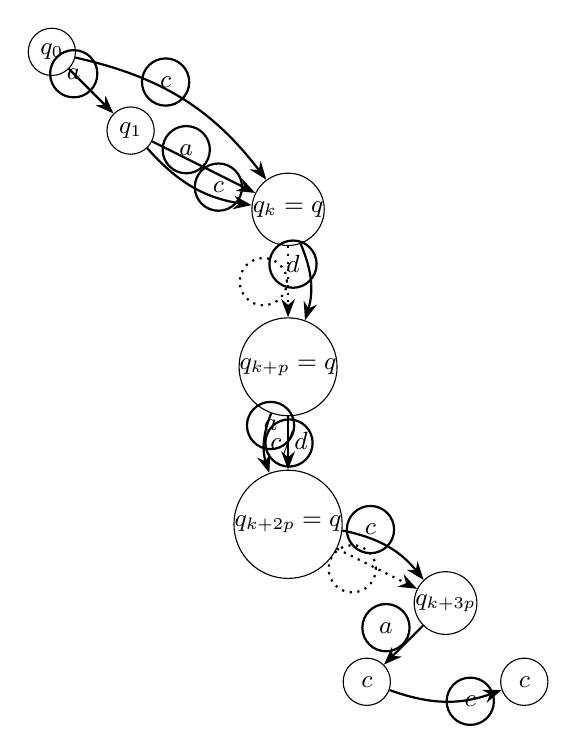
\begin{tikzpicture}[>=Stealth, node distance=2cm, auto, scale=1]

% Node styles
\tikzset{
    every node/.style={
        draw,
        shape=circle,
        minimum size=6mm,
        inner sep=0pt,
        font=\small
    },
    every edge/.style={
        draw,
        thick
    }
}

% Nodes definition
\node (q0) at (0, 0) {$q_0$};
\node (q1) at (1, -1) {$q_1$};
\node (qk) at (3, -2) {$q_k = q$};
\node (qkp) at (3, -4) {$q_{k+p} = q$};
\node (qk2p) at (3, -6) {$q_{k+2p} = q$};
\node (qk3p) at (5, -7) {$q_{k+3p}$};
\node (end1) at (6, -8) {$c$};
\node (end2) at (4, -8) {$c$};

% Edges definition
\path[->] 
    (q0) edge node[above left] {$a$} (q1)
    (q1) edge node[above left] {$a$} (qk)
    (qk) edge[dotted] node[left] {} (qkp)
    (qkp) edge node[above left] {$a$} (qk2p)
    (qk2p) edge[dotted] node[left] {} (qk3p)
    (qk3p) edge node[above left] {$a$} (end2);

\path[->] 
    (q0) edge[bend left=20] node[above left] {$c$} (qk)
    (q1) edge[bend right=20] node[right] {$c$} (qk)
    (qk) edge[bend left=20] node[above left] {$d$} (qkp)
    (qkp) edge[bend right=20] node[right] {$c/d$} (qk2p)
    (qk2p) edge[bend left=20] node[above left] {$c$} (qk3p)
    (end2) edge[bend right=20] node[right] {$c$} (end1);

\end{tikzpicture}
\end{document}